\documentclass{article}

\usepackage[utf8]{inputenc}
\usepackage[T1]{fontenc}
\usepackage{polski}
\usepackage{indentfirst}
\usepackage{lastpage}
\usepackage{natbib}
\usepackage{graphicx} 
\usepackage{sidecap}
\usepackage{wrapfig}
\usepackage{subfig}
\usepackage{caption}



\usepackage{fancyhdr}
\pagestyle{fancy}
\fancyhf{}
\rhead{Franciszek Wysocki}
\rfoot{Strona \thepage \hspace{1pt} z \pageref{LastPage}}
\lhead{Spis treści}
\title{Specyfikacja funkcjonalna projektu pt. ,,Centrum Zarządzania Szczepionkami''}
\author{}
\date{}

\begin{document}
\maketitle

\begin{flushright}
\par
\vfill
\par
{\fontsize{11}{11}\selectfont
    Wykonał: Franciszek Wysocki

    Sprawdzający: mgr inż. Paweł Zawadzki

    Data: 08-11-2020
}
\end{flushright}
\thispagestyle{empty}

\newpage

\tableofcontents

\newpage

\section{Cel dokumentu}
{\fontsize{12}{12}\selectfont

    Celem dokumentu jest przedstawienie funkcjonalności programu zarządzającego dostawami szczepionek. Zostanie zaprezentowany sposób, w jaki aplikacja powinna być uruchamiana, plik wejściowy wymagany do uruchomienia oraz plik wyjściowy zawierający dane wynikowe działania programu. Zostaną również opisane sytuacje nieporządane, jak i reakcja na nie.

}

\lhead{Cel dokumentu}

\section{Cel projektu}
{\fontsize{12}{12}\selectfont
    Celem projektu jest zapewnienie optymalnego sposobu dostaw szczepionek poprzez opracowanie odpowiedniego programu. Ten, dokonując analizy konkretnych danych, dostarczonych przez grupę menadżerską, powinien doprowadzić do ustalenia w jaki sposób należy przeprowadzić dostawy, aby możliwie wypełnić dzienne zapotrzebowanie wszystkich zarządzanych aptek, robiąc to jednocześnie przy najmniejszym możliwym koszcie całkowitym.
    Uzykane wnioski, informujące o tym, która apteka powinna zamówić jaką ilość szczepionek od którego producenta, powinny zostać zapisane do pliku wyjściowego.

}

\section{Sposób wywołania programu}
{\fontsize{12}{12}\selectfont
    Aplikacja powinna być wywoływana w konsoli, ze względu na brak interfejsu graficznego oraz wyświetlające się ewentualne komunikaty o błędach. Aby uruchomić program można wykorzystać poniższą komendę, podmieniając odpowiednie nazwy.
    
    \begin{center}
        \texttt{java -jar nazwaProgramu.jar nazwaPlikuWejściowego.txt} 
    \end{center}
  
   
    \setlength{\parindent}{0pt}
    Plik wejściowy należy umieścić w tym samym katalogu, w jakim znajduje się program.
    \setlength{\parindent}{12pt}
    \newline
    
    Komputer uruchamiający aplikacje powinien posiadać zainstalowane JDK. Zależnie od systemu powinna również zostać skonfigurowana odpowiednia zmienna środowiskowa, aby powyższa komenda była rozpoznawana.
}

    


\section{Dane wejściowe}
{\fontsize{12}{12}\selectfont
    Plik wejściowy, wymagany do uruchomienia programu, powinien być w formacie tekstowym o rozszerzeniu txt. Podanie nazwy pliku jest wymagane jako argument polecenia wywołującego program (Nazwa może być dowolna).

    
    Przykładowa treść pliku:
    
    \begin{figure} [hbt!]
        \centering
        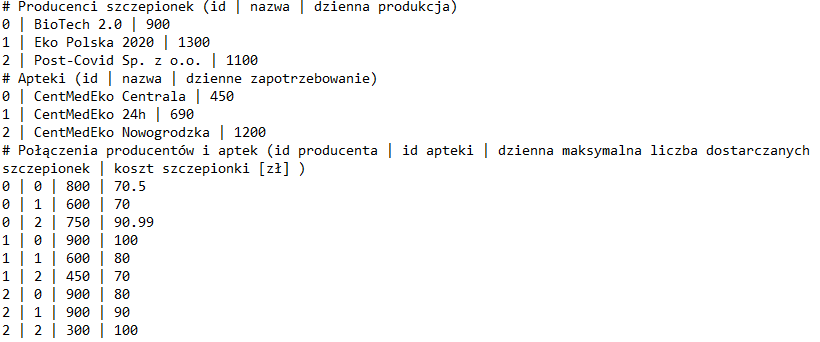
\includegraphics[width=13.5cm]{input.png}
      \captionof{figure}{}
    \end{figure}
    
    Uwagi i zastrzeżenia:
    \begin{itemize}
     \item Numer identyfikacyjny (id) powinien być liczbą całkowitą indywidualną w danej kategorii.
     \item Symbol odzielenia kolejnych elementów powinien składać się z trzech znaków, kolejno: spacji, kreski pionowej i kolejnej spacji -> ,, | ''.
     \item Liczby reprezentujące dzienną produkcję, dzienne zapotrzebowanie i dzienną maksymalną liczbę dostarczonych szczepionek powinny być liczbami naturalnymi. Cena natomiast powinna być dodatnią liczbą zmiennoprzecinkową.
     \item Nagłowki mogą się różnić (muszą jednak istnieć i zaczynać się od symbolu ,,\#'', gdyż to one rozpoczynają kolejną kategorię danych - stąd w danym pliku powinny istnieć trzy).
     \item Zarówno kolejność kategorii, jak i kolejność danych powinna być zgodna z powyższym przykładem (kolejność kategorii: producenci, apteki, połączenia, kolejność danych zgodna z nawiasami w komentarzach).
     \item Powinno istnieć połączenie każdego producenta z każdą apteką (lecz nie powinno istnieć więcej niż jedno dla danej pary).
    
    \end{itemize}
    \lhead{Dane wejściowe}
    
    Niedopełnienie któregokolwiek z powyższych podpunktów, będzie skutkowało wyświetleniem komunikatu i przerwaniem pracy programu. 
}

\newpage
\section{Dane wyjściowe}
{\fontsize{12}{12}\selectfont
    Dane wyjściowe zostaną utworzone w formacie tekstowym o rozszerzeniu txt. Nazwa pliku zostanie stworzona łącząc nazwę pliku wejściowego ze słowem ,,output'' nadpisując plik, jeśli w danej lokalizacji już istnieje o identycznej nazwie.
    
    Przykładowa treść pliku:

    \begin{figure} [hbt!]
        \centering
        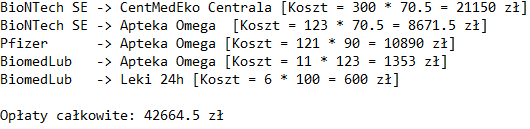
\includegraphics[width=12cm]{output.png}
      \captionof{figure}{}
    \end{figure}
    
\lhead{Dane wyjściowe}

    Uwagi:
    \begin{itemize}
        \item Każda linijka składa się z czterech kolejnych elementów:
            \begin{itemize}
                \item nazwa producenta
                \item symbol oddzielenia (kolejno: spacja, strzałka ,, -> '', spacja) wyrównany do najdłuższej nazwy producenta.
                \item nazwa apteki
                \item koszt (podany w nawiasie kwadratowym).
            \end{itemize}
        \item Na końcu pliku znajduje się podsumowanie całkowitego kosztu.
        \item Zamówienia, w których liczba zamówionych szczepionek wyniosła zero nie będą zapisywane.
    
    \end{itemize}
}
\section{Przykładowy scenariusz uruchomienia}

{\fontsize{12}{12}\selectfont
    
    Użytkownik uruchamia terminal i przechodzi do katalogu, w którym znajduje się program. Następnie uruchamia go zgodnie z punktem ,,Sposób wywołania programu'', podając jako argument nazwę pliku z danymi. Następuje weryfikacja poprawności danych, po czym rozpoczyna się przygotowywanie odpowiedniej konfiguracji. Po zakończeniu tego procesu wynik zostaje zapisany do pliku tekstowego.
    
    W razie wystąpienia błędu, na terminalu użytkownika pojawi się specjalny komunikat z informacją o błędzie i program zakończy działanie. Gdy użytkownik poprawi błąd, proces powinien rozpocząć od początku.


}

\section{Komunikaty o błędach}
{\fontsize{12}{12}\selectfont
    Komunikaty o błędach będą wyświetlane w konsoli.
    Może to nastąpić między innymi w następujacych sytuacjach:
    
   \begin{itemize}
        \item Brak argumentu wywołania.
        \item Zbyt wiele argumentów wywołania.
        \item Podany plik nie istnieje.
        \item Niepoprawne rozszerzenie pliku.
        \item Niepoprawne ułożenie danych (np. brak nagłówków, zmiana kolejności danych, itd...)
        \item Niepoprawne dane (np. cena ujemna).
        \item Nieporawna ilość danych.
        \item Błąd zapisu danych (np. chroniona lokalizacja).
        \item Inne błędy systemowe.
   \end{itemize}
   
   Komunikaty będą stworzone w taki sposób, aby ułatwić lokalizację nastąpił problemu.
   Każdy błąd kończy działanie programu, aby nie doprowadzić do wieloznacznych (nieporządanych) sytuacji.


}
\lhead{Komunikaty o błędach}

\end{document}
